%% LaTeX-Beamer template for KIT design
%% by Erik Burger, Christian Hammer
%% title picture by Klaus Krogmann
%%
%% version 2.1
%%
%% mostly compatible to KIT corporate design v2.0
%% http://intranet.kit.edu/gestaltungsrichtlinien.php
%%
%% Problems, bugs and comments to
%% burger@kit.edu

\documentclass[18pt]{beamer}

\usepackage[utf8]{inputenc}
\usepackage[babel,german=quotes]{csquotes}
\usepackage{graphicx}
\usepackage{caption}
\usepackage{subfig}
\usepackage[right]{eurosym}
\usepackage{listings}

%% SLIDE FORMAT

% use 'beamerthemekit' for standard 4:3 ratio
% for widescreen slides (16:9), use 'beamerthemekitwide'

\usepackage{templates/beamerthemekit}
% \usepackage{templates/beamerthemekitwide}

%% TITLE PICTURE

% if a custom picture is to be used on the title page, copy it into the 'logos'
% directory, in the line below, replace 'mypicture' with the 
% filename (without extension) and uncomment the following line
% (picture proportions: 63 : 20 for standard, 169 : 40 for wide
% *.eps format if you use latex+dvips+ps2pdf, 
% *.jpg/*.png/*.pdf if you use pdflatex)

\titleimage{title}

%% TITLE LOGO

% for a custom logo on the front page, copy your file into the 'logos'
% directory, insert the filename in the line below and uncomment it

\titlelogo{titlelogo}

% (*.eps format if you use latex+dvips+ps2pdf,
% *.jpg/*.png/*.pdf if you use pdflatex)

%% TikZ INTEGRATION

% use these packages for PCM symbols and UML classes
% \usepackage{templates/tikzkit}
% \usepackage{templates/tikzuml}

% the presentation starts here

\title[C++ Workshop]{C++ Workshop}
\subtitle{1. Block, 27.04.2012}
\author{Markus Jung, Christian Käser, Robert Schneider}

\institute{}

\begin{document}

% change the following line to "ngerman" for German style date and logos
\selectlanguage{ngerman}

\AtBeginSection[]{%
	\begin{frame}
		\tableofcontents[sectionstyle=show/hide,subsectionstyle=hide/show/hide]
	\end{frame}
	\addtocounter{framenumber}{-1}% If you don't want them to affect the slide number
}

%title page
\begin{frame}
\titlepage
\end{frame}

%table of contents
\begin{frame}{Gliederung}
\tableofcontents
\end{frame}

\section{Organisatorisches}


\subsection{Platzzahl}

\begin{frame}{Begrenzung der Platzzahl}
	\begin{block}{Warum eine Begrenzung?}
		\begin{itemize}
			\item Raumgröße
			\item Betreuung, Gruppengröße
		\end{itemize}
	\end{block}
	\ \\
	\pause
	\ \\
	\begin{block}{Platzzahl}
		\begin{itemize}
			\item Max. 24 Plätze, Betreuer zusätzlich
			\item Warteschlange (wie bei Sprachkurs)
			\item Online-Teilnahme möglich
			\begin{itemize}
				\item Die Vorträge werden (versuchsweise) als Screencast aufgezeichnet
				\item Fragen können über die Mailinglist gestellt werden
				\item \dots oder über unseren IRC-Channel
			\end{itemize}
		\end{itemize}
	\end{block}
\end{frame}

\begin{frame}[fragile]{Wie bekomme ich einen Platz?}
	Nach folgenden Kriterien werden die Plätze verteilt:
	\begin{enumerate}
		\item Anwesenheit heute (27.4.) oder Entschuldigung
		\item Erforderliche Programmierkenntnisse
		\begin{itemize}
			\item \enquote{Programmieren für Physiker} als Referenz
			\item Codebeispiel zum ersten Termin in \verb|example_apps/easy.cpp| als Minimalanforderung
		\end{itemize}
		\item Aktive Teilnahme und Interesse (der \emph{Willen}, teilzunehmen und das durchzuziehen)
		\item first-come, first-served (Wer zuerst kommt, mahlt zuerst.)
	\end{enumerate}
	
	Nachrücken ist möglich!
\end{frame}



\subsection{Organisatorisches}

\begin{frame}{Kontakt, Kooperation}
	\begin{description}
		\item[Mailing-List] cpp-workshop@lists.kit.edu
		\item[IRC] \#kit-cpp-workshop auf irc.euirc.net
		\item[GitHub]	\url{www.github.com}, Organization kit-cpp-workshop
	\end{description}
	\ \\
	
	Namen und E-Mail-Adressen:
	\begin{table}
		\begin{tabular}{l|l}
			Christian Käser	&	Christian.Kaeser@student.kit.edu	\\
			\hline
			Markus Jung		&	Markus.Jung@stud.uni-karlsruhe.de	\\
			\hline
			Matthias Blaicher	&	matthias@blaicher.com	\\
			\hline
			Robert Schneider	&	Robert.Schneider3@student.kit.edu	\\
			\hline
			Sven Brauch	&	SvenBrauch@googlemail.com	\\
		\end{tabular}
	\end{table}
\end{frame}

\begin{frame}{Der Workshop}
	\begin{block}{Termin}
		\begin{itemize}
			\item jeden Freitag in der Vorlesungszeit
			\item 15:45-17:15
			\item Raum: 2-0 (Physik-Hochhaus)
			\item evtl. Zusatztermine nach Absprache (z.B. cmake)
		\end{itemize}
	\end{block}
	\pause
	\begin{block}{Ziele}
		\begin{itemize}
			\item Erfahrungsaustausch!
			\item Hilfe zur Selbsthilfe / Anhaltspunkte zum Weiterlernen
			\item Tiefergehenderer Einblick in die Sprache
			\item Verschiedene Gebiete von C++ (\enquote{Schweizer Taschenmesser})
			\item Kooperation, Team-Programmierung
			\item Software-Design, programming idioms, Fehler vermeiden usw.
		\end{itemize}
	\end{block}
\end{frame}

\begin{frame}{Struktur eines Workshops}
	\begin{block}{Themen}
		\begin{itemize}
			\item Richten sich nach den Interessen der Teilnehmer!
			\item Grundlegende Methodiken, Werkzeuge, ...
			\item Objektorientierung
			\item Algorithmen \& Datenstrukturen
			\item Verwendung von Bibliotheken (statisch, dynamisch gelinkt)
		\end{itemize}
	\end{block}
	\pause
	\begin{block}{Aufteilung}
		\begin{itemize}
			\item Theoretischer Teil, heute: Organisatorisches, git, eclipse
			\item Praktischer Teil: pair programming (2er-Teams) IDE + hello-world
			\item Übungen: im praktischen Teil, zu Hause fertig. Vorstellung einiger Lösungen in darauffolgender Woche
		\end{itemize}
	\end{block}
\end{frame}


\section{Versionsverwaltung}
\subsection{Motivation}
\begin{frame}{Motivation}
	\begin{itemize}
		\item \enquote{Gestern ging es noch \dots}
		\item \enquote{Das Problem hatten wir doch schon Mal \dots}
		\item \enquote{Wer hat den ?\&(\%!\$ verzapft!?}
	\end{itemize}
	\ \\
	\pause
	\ \\
	\begin{block}{Aufgaben}
		\begin{itemize}
			\item Archivierung der Entwicklungsgeschichte
			\begin{itemize}
				\item \enquote{Zeitmaschine}
			\end{itemize}
			\item Koordination paralleler Entwicklungsvorgänge
		\end{itemize}
	\end{block}
\end{frame}

\subsection{Konzepte}
\begin{frame}{Konzepte I}
	\begin{block}{Version/Revision/Commit}
		Eine Momentaufnahme der verwalteten Dateien, verknüpft mit Metadaten wie Autor, Datum und einer Beschreibung
	\end{block}
	\begin{block}{Versionsgeschichte}
		Stellt den Bezug zwischen einzelnen Versionen her
	\end{block}
	\begin{block}{Repository}
		Speichert und verwaltet die Versionsgeschichte sowie die zugehörigen Versionen
	\end{block}
	\begin{block}{Arbeitskopie}
		Ein Abbild einer Version im Dateisystem, an dem auch Änderungen vorgenommen werden können
	\end{block}
\end{frame}
\begin{frame}{Konzepte I}
	\begin{figure}
		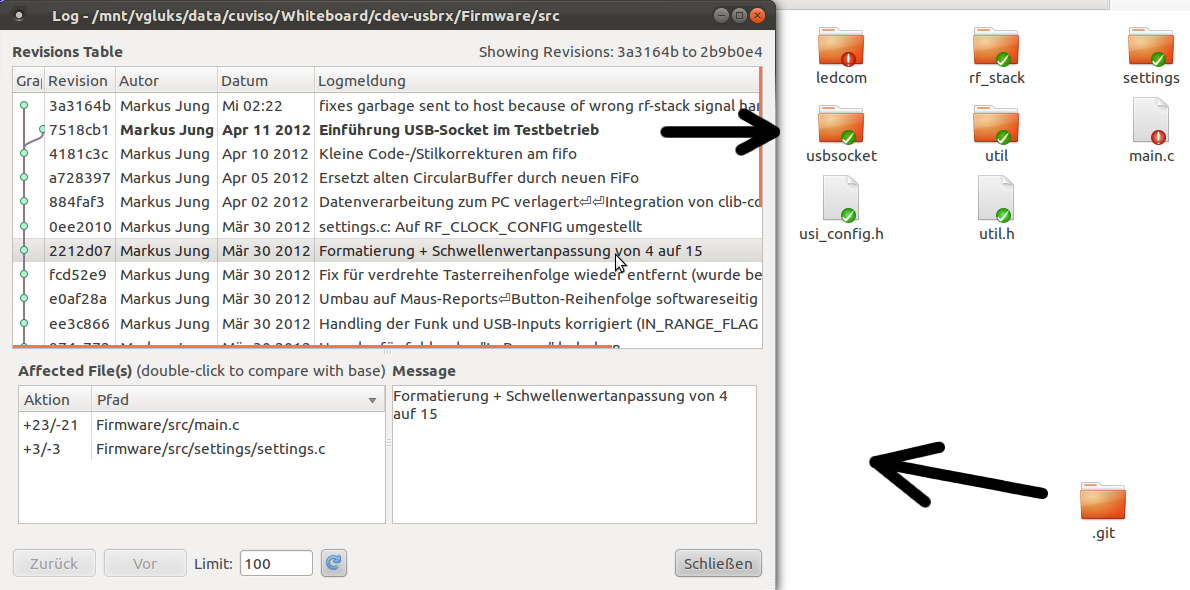
\includegraphics[width=\linewidth]{images/history.png}
	\end{figure}
\end{frame}
\begin{frame}{Konzepte II}
	\begin{columns}
		\column{.1\linewidth}
			\begin{figure}
				
\includegraphics[width=\linewidth]{images/branchmerge.png}
			\end{figure}

		\column{.9\textwidth}
			\begin{block}{Dezentral}
				\begin{itemize}
					\item Jeder Nutzer hat ein (lokales) Repository \\
					\item Erfordert keinen kontinuierlichen Zugriff auf den Server
				\end{itemize}
			\end{block}
			\begin{block}{Branch}
				\begin{itemize}
					\item Softwareentwicklung ist selten linear (\enquote{Entwicklungszweig})
					\item Versionsverwaltungen bilden das durch \enquote{branches} ab
				\end{itemize}
			\end{block}
			\begin{block}{Merge}
				\begin{itemize}
					\item Führt Entwicklungszweige zusammen
					\item Konkurrierende Änderungen können Konfliktlösung erfordern
				\end{itemize}
			\end{block}
			\begin{block}{Tag}
				Markiert Versionen zum schnellen Zugriff
			\end{block}
\end{columns}
\end{frame}

\subsection{GIT}
\begin{frame}{GIT Workflow}
	\begin{figure}
		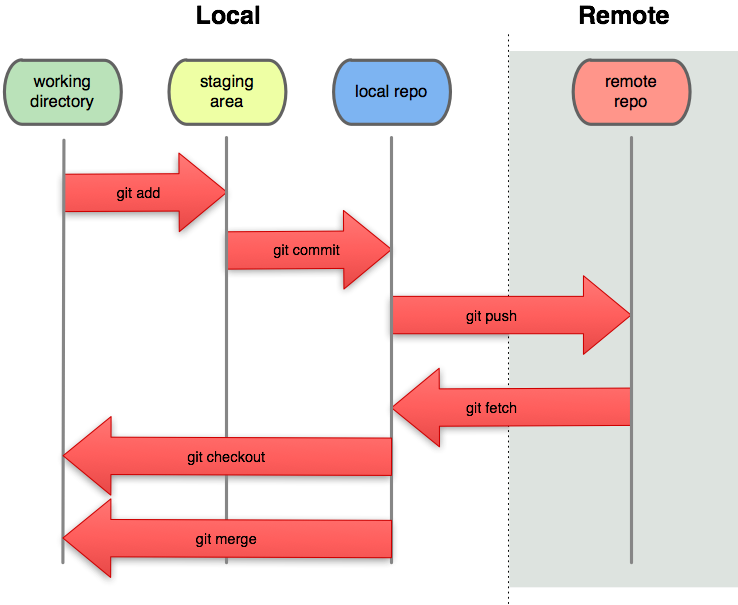
\includegraphics[width=0.75\linewidth]{images/local-remote.png}
	\end{figure}
\end{frame}

\begin{frame}[fragile,allowframebreaks]{GIT Referenz}
	\begin{block}{Repository erzeugen}
		\begin{itemize}
			\item Leeres neues Repository: \verb|git init [<Ordnername>]|
			\item Kopie eines existierenden Repositories: \verb|git clone <URL> [<Ordnername>]|
		\end{itemize}
	\end{block}
	\begin{block}{Änderungen vornehmen}
		\begin{itemize}
			\item Neue/geänderte Datei für die nächste Revision vormerken: \verb|git add <Datei/Ordner>|
			\item Datei aus der Versionskontrolle entfernen: \verb|git rm [--cached] [-r] <Datei/Ordner>|
			\item Vorgemerkte Änderungen verwerfen: \verb|git reset <Datei/Ordner>|
			\item Änderungen übernehmen (neue Revision erzeugen): \verb|git commit [-m "commit message"]| \\
				Commit-Message-Styleguide:
			\begin{itemize}
				\item Eine Zeile Kurzzusammenfassung
				\item Danach ggf. eine Leerzeile und weiterer Text
				\item Zeilenlänge $\le$ 72 Zeichen
			\end{itemize}
		\end{itemize}
	\end{block}
	\begin{block}{Austausch mit anderen Repositories}
		\begin{itemize}
			\item Änderungen an externes Repository übertragen: \verb|git push [--all] [--tags] [<Repository>] [<Branch>]|
			\item Änderungen aus externem Repository beziehen: \verb|git fetch [<Repository>]|
			\item Änderungen aus externem Repository beziehen und anwenden: \verb|git pull [<Repository>]|
			\item Verwaltung externer Repositories: \verb|git remote|
		\end{itemize}
	\end{block}
	\begin{block}{Verzweigungen und ähnlicher Wildwuchs}
		\begin{itemize}
			\item Aktuelle Revision/Branch der Arbeitskopie wechseln: \verb|git checkout [-b] [<Branch>]|
			\item Verwaltung von Branches: \verb|git branch|
			\item Zweig mit eigenem zusammenführen: \verb|git merge <Branch>|
			\item Tagging: \verb|git tag <Tag> [<Revision>]|
		\end{itemize}
	\end{block}
\end{frame}

\begin{frame}[fragile]{GIT und github}
	\begin{block}{github}
		\begin{itemize}
			\item Hosting für GIT-Repositories
			\item Für Open-Source-Entwicklung kostenlos
			\item \enquote{social coding}
		\end{itemize}
	\end{block}
	\begin{block}{Fork}
		\begin{itemize}
			\item Eine Abspaltung eines GIT-Repositories
			\begin{itemize}
				\item Jeder \verb|clone| eines Repositories ist eigentlich ein Fork
			\end{itemize}
			\item Eigene Entwicklung finden im eigenen Fork statt
		\end{itemize}
	\end{block}
	\begin{block}{Pull-Request}
		\begin{itemize}
			\item Aufforderung an den Besitzer eines externen Repositories, Änderungen zu übernehmen
		\end{itemize}
	\end{block}
\end{frame}

\subsection{Weiterführende Hinweise}
\begin{frame}[fragile]{Hilfe zur Selbsthilfe}
	\begin{itemize}
		\item \verb|man git| beziehungsweise \verb|git help|
		\item \url{http://help.github.com/} - Github Hilfe
		\item \url{http://www.youtube.com/watch?v=4XpnKHJAok8} \\
			Google Talk "Linus Torvalds on Git"
		\item \url{http://git-scm.com/} - Offizielle Website
	\end{itemize}
\ \\

\tiny
	\begin{itemize}
		\item \url{https://github.com/Gazler/githug} - Interaktives Git Tutorial
		\item \url{http://gitref.org/} - Git Referenz
		\item \url{http://progit.org/book/} - The Pro Git Book
		\item \url{http://gitready.com/} - Git tips and tricks
	\end{itemize}
\end{frame}

\subsection{Aufgaben}
\begin{frame}[fragile]{Aufgaben}
	\begin{itemize}
		\item Github: Aufgaben forken, zum clonen HTTPS (statt SSH) nutzen
		\item \verb|git clone https://...|
		\item Änderungen machen
		\item \verb|git add dateiname|
		\item \verb|git commit|
		\item \verb|git push|
	\end{itemize}
\end{frame}

\section{Entwicklungsumgebung}
\begin{frame}{Was ist eine Entwicklungsumgebung?}
	\begin{block}{IDE}
		Integrated Development Environment
	\end{block}
	\pause
	\begin{block}{Sammlung \emph{und Integration} von Werkzeugen}
		\begin{itemize}
			\item intelligenter Texteditor
			\item grafischer Debugger
			\item Autovervollständigung
			\item einfache Anbindung an den Compiler
			\item Hilfefunktion
			\item meist erweiterbar (z.B. git-Integration)
		\end{itemize}
	\end{block}
\end{frame}

\begin{frame}{Wofür?}
	\begin{description}
		\item[\textbf{grafisch}] IDEs sind üblicherweise grafisch, man kann daher viele Dinge über GUIs konfigurieren und anstoßen
		\item[\textbf{integriert}] es werden zahlreiche Werkzeuge miteinander vereint, z.B. ein Text-Editor mit einem Debugger
		\item[\textbf{strukturiert}] in der IDE wird zumeist auch die Struktur eines Projektes abgebildet (Ressourcen, source code usw.)
		\item[\textbf{editor}] die IDE kennt das gesamte Projekt und kann daher die Informationen aus allen Dateien nutzen (autocompletion, definition lookup etc.)
		\item[\textbf{code analysis}] durch ihre umfassendes Wissen kann die IDE auch den code analysieren, etwa um die Struktur von Klassen darstellen zu können
		\item[\textbf{refactoring}] das Umstrukturieren von code ist in gewissen Grenzen ebenfalls automatisiert möglich
	\end{description}
\end{frame}

\begin{frame}{Beispiele}
	\begin{itemize}
		\item Code::Blocks
		\item \emph{Eclipse}
		\item GNU Emacs
		\item KDevelop
		\item NetBeans
		\item Qt Creator
		\item proprietär: Visual Studio (Microsoft / Windows)
		\item proprietär: Xcode (Apple / OS~X, iOS)
		\item \dots
	\end{itemize}
\end{frame}
\section{Praxis}
\begin{frame}[fragile]{Und jetzt: Praxis!}
	\begin{itemize}
		\item Aufgabe 1: Hello World
		\item Aufgabe 2: Fibonacci-Zahlen
		\item Bonusaufgabe: Project Euler
	\end{itemize}
	\ \\
	\ \\
	URL zum Workshop: \\
	\large{\url{https://github.com/kit-cpp-workshop/workshop-ss12-01}} \\
	\ \\
	Die Aufgabenbeschreibungen und weiterführende Hinweise enthält die Datei \verb|README.md|\\
\end{frame}


\end{document}
